% IEEE Paper Template for US-LETTER Page Size (V1)
% Sample Conference Paper using IEEE LaTeX style file for US-LETTER pagesize.
% Copyright (C) 2006-2008 Causal Productions Pty Ltd.
% Permission is granted to distribute and revise this file provided that
% this header remains intact.
%
% REVISION HISTORY
% 20080211 changed some space characters in the title-author block
%
% \documentclass[10pt,conference,letterpaper]{IEEEtran}
% \usepackage{times,amsmath,epsfig}
% \usepackage[utf8]{inputenc}
% \usepackage[usenames,dvipsnames]{color}
% \usepackage{amssymb}

\documentclass[a4paper,english]{llncs}
\usepackage[T1]{fontenc}
\usepackage[latin9]{inputenc}
\usepackage{lmodern}
\usepackage{float}
\usepackage{slashed}
\usepackage{graphicx}
\usepackage{fixltx2e}
\usepackage{amsmath}
\usepackage{epstopdf}
\usepackage{url}
\usepackage{seqsplit} % for splitting very long variable names
\usepackage[dvipsnames]{xcolor}
\usepackage{listings}

\hyphenation{bio-ban-kers}
\hyphenation{Bio-bank-Cloud}

\newcommand\YAMLcolonstyle{\color{black}}
\newcommand\YAMLkeystyle{\color{blue}}
\newcommand\YAMLvaluestyle{\color{black}}

% \newcommand\language@yaml{yaml}
% 
% \expandafter\expandafter\expandafter\lstdefinelanguage
% \expandafter{\language@yaml}
% {
%   keywords={name,ec2,type,region,cookbooks,groups,size,recipes,github,branch},
%   keywordstyle=\color{blue}\bfseries,
%   basicstyle=\color{black},                                 % assuming a key comes first
%   sensitive=false,
%   comment=[l]{\#},
%   morecomment=[s]{/*}{*/},
%   commentstyle=\color{purple}\ttfamily,
%   stringstyle=\YAMLvaluestyle\ttfamily,
%   moredelim=[l][\color{orange}]{\&},
%   moredelim=[l][\color{magenta}]{*},   % switch to value style at :
%   literate =    {---}{{\ProcessThreeDashes}}3
%                 {>}{{\textcolor{red}\textgreater}}1     
%                 {|}{{\textcolor{red}\textbar}}1 
%                 {\ -\ }{{\mdseries\ -\ }}3,
% }
% 
% % switch to key style at EOL
% \lst@AddToHook{EveryLine}{\ifx\lst@language\language@yaml\YAMLkeystyle\fi}
% % \makeatother
% 
% \newcommand\ProcessThreeDashes{\llap{\color{cyan}\mdseries-{-}-}}
% 
% \usepackage{hyperref}
% \newcommand\fnurl[2]{%
% \footnote{\label{#1}\href{#2}{#2}}%
% }
% 



\makeatletter
\raggedbottom % remove unwanted space between paragraphs 

%%%%%%%%%%%%%%%%%%%%%%%%%%%%%% LyX specific LaTeX commands.
\pdfpageheight\paperheight
\pdfpagewidth\paperwidth

\floatstyle{ruled}
\newfloat{algorithm}{tbp}{loa}
\providecommand{\algorithmname}{Algorithm}
\floatname{algorithm}{\protect\algorithmname}

%%%%%%%%%%%%%%%%%%%%%%%%%%%%%% User specified LaTeX commands.
\usepackage{paralist}
\usepackage[noend]{algorithm,algcompatible,algpseudocode}
\usepackage{amssymb} % for symbols 
\usepackage{caption} % algorthm is a float and does not split. use caption instead
% \usepackage{subcaption}
\usepackage{etoolbox}\AtBeginEnvironment{algorithmic}{\footnotesize}
%\algsetup{linenosize=\small}
\usepackage{subfig}
\usepackage[T1]{fontenc}
\usepackage{mwe}    % loads »blindtext« and »graphicx«

\makeatother
\algblockdefx[NAME]{StartTransaction}{EndTransaction}
[1]{\textbf{begin transaction} \textbf{#1}}{\textbf{commit transaction}}
\algrenewcommand\alglinenumber[1]{\footnotesize #1:}

\usepackage{babel}
\usepackage{cite}
\usepackage{amssymb}% http://ctan.org/pkg/amssymb
\usepackage{pifont}% http://ctan.org/pkg/pifont
\newcommand{\cmark}{\ding{51}}%
\newcommand{\xmark}{\ding{53}}%

\title{BiobankCloud: a Platform for the Secure Storage, Sharing, and Processing of Large Biomedical Data Sets}

\author{Alysson Bessani\inst{5}, J\"{o}rgen Brandt\inst{2}, Marc Bux\inst{2}, Vinicius Cogo\inst{5}, Lora Dimitrova\inst{4}, Jim Dowling\inst{1}, Ali Gholami\inst{1}, Kamal Hakimzadeh\inst{1}, Micheal Hummel\inst{4}, Mahmoud Ismail\inst{1}, Erwin Laure\inst{1}, Ulf Leser\inst{2}, Jan-Eric Litton\inst{3}, Roxanna Martinez\inst{3}, Salman Niazi\inst{1}, Jane Reichel\inst{6}, Karin Zimmermann\inst{4}}

\institute{KTH - Royal Institute of Technology,\\
\email{\{jdowling, gholami, mahh, maism, erwinl, smkniazi\}@kth.se}
\and
Humboldt University\\
\email{\{leser, bux, joergen.brandt\}@informatik.hu-berlin.de}
\and
Karolinska Institute\\
\email{\{Jan-Eric.Litton, Roxanna.Martinez\}@ki.se}
\and
Charite\\
\email{\{Michael.Hummel, Lora.Dimitrova, Karin.Zimmermann\}@charite.de}
\and
LaSIGE, Faculdade de Ci\^{e}ncias, Universidade de Lisboa, Portugal\\
\email{\{bessani, vielmo\}@lasige.di.fc.ul.pt}
\and
Uppsala University\\
\email{\{jane.reichel\}@jur.uu.se}
}

\newif\ifshowcomments
\showcommentstrue

\ifshowcomments
\newcommand{\mynote}[2]{\fbox{\bfseries\sffamily\scriptsize{#1}}
{\small$\blacktriangleright$\textsf{\emph{#2}}$\blacktriangleleft$}}
\else
\newcommand{\mynote}[2]{}
\fi
\newcommand{\jim}[1]{\textcolor{Red}{\mynote{Jim}{#1}}}

\begin{document}
\maketitle

\begin{abstract}
Biobanks store and catalog human biological material that is increasingly being digitized using next-generation sequencing (NGS). There is, however, a computational bottleneck, as existing software systems are not scalable and secure enough to store and process the incoming wave of genomic data from NGS machines. In the BiobankCloud project, we are building a Hadoop-based platform for the secure storage, sharing, and parallel processing of genomic data. We extended Hadoop to include support for multi-tenant studies, reduced storage requirements with erasure coding, and added support for extensible and consistent metadata. On top of Hadoop, we built a scalable scientific workflow engine featuring a proper workflow definition language focusing and simple integration and chaining of existing tools, adaptive scheduling on Apache Yarn, and support for iterative dataflows. Our platform also supports the secure sharing of data across different, distributed Hadoop clusters. The software is easily installed and comes with a provide user-friendly web interface for running, managing, and accessing data sets behind a secure 2-factor authentication. Initial tests have shown that the engine scales well to dozens of nodes. The entire system is open-source and includes pre-defined workflows for popular tasks in biomedical data analysis, such as variant identification, differential transcriptome analysis using RNA-Seq, and analysis of miRNA-Seq, and ChIP-Seq data.
\end{abstract}

%\vskip-5pt

\section{Introduction}
Biobanks store and catalog human biological material from identifiable individuals for both clinical and research purposes. Recent initiatives in personalized medicine created a steeply increasing demand to sequence the human biological material stored in biobanks. As of 2015, such large-scale sequencing is under way in hundreds of projects around the world, with the largest single project sequencing up to 100.000 genomes\footnote{See \url{http://www.genomicsengland.co.uk/}.}. Furthermore, sequencing also is becoming more and more routine in a clinical setting for improving diagnosis and therapy especially in cancer\cite{pmedicine}. However, software systems for biobanks traditionally managed only metadata associated with samples, such as pseudo-identifiers for patients, sample collection information, or study information. Such systems cannot cope with the current requirement to, alongside such metadata, also store and analyze genomic data, which might mean everything from a few Megabytes (e.g., genotype information from a SNP array) to hundreds of Gigabytes per sample (for whole genome sequencing with high coverage). 

For a long time, such high-throughput sequencing and analysis was only available to large research centers that (a) could afford enough modern sequencing devices and (b) had the budget and IT expertise to manage high performance computing clusters. This situation is changing. The cost of sequencing is falling rapidly, and more and more labs and hospitals depend on sequencing information for daily research and diagnosis/treatment. However, there is still a pressing need for flexible and open software systems to enable the computational analysis of large biomedical data sets at a reasonable price. Note that this trend is not restricted to genome sequencing; very similar developments are also happening in other medical areas, such as molecular imaging\cite{imaging}, drug discovery\cite{drug}, or data generated from patient-attached sensors\cite{qself}. 

In this paper, we present the BiobankCloud platform, a collaborative project bringing together computer scientists, bioinformaticians, pathologists, and biobankers. The system is designed as a ``platform-as-a-service'', i.e., it can be easily installed on a local cluster (or, equally well, in a public cloud) using Karamel and Chef\footnote{\url{http://www.karamel.io}}. Primary design goals are flexibility in terms of the analysis being performed, scalability up to very large data sets and very large cluster set-ups, ease of use and low maintenance cost, strong support for data security and data privacy, and direct usability for users. To this end, it encompasses (a) a scientific workflow engine running on top of the popular Hadoop platform for distributed computing, (b) a scientific workflow language focusing on easy integration of existing tools and simple rebuilding of existing pipelines, (c) support for automated installation, and (d) role-based access control. It also features (e) HopsFS, a new version of Hadoop's Distributed Filesystem (HDFS) with improved throughput, supported for extended metadata, and reduced storage requirements compared to HDFS, (f) Charon, which enables the federation of clouds at the file system level, and (g) a simple Laboratory Information Management Service with an integrated web interface for authenticating/authorizing users, managing data, designing and searching for metadata, and support for running workflows and analysis jobs on Hadoop. This web interface hides much of the complexity of the Hadoop backend, and supports multi-tenancy through first-class support for \textit{Studies}, \textit{SampleCollections} (DataSets), \textit{Samples}, and \textit{Users}. 

In this paper, we give an overview on the architecture of the BiobankCloud platform and describe each component in more detail. The system is currently under development; while a number of components already have been released for immediate usage (e.g., Hops, SAASFEE), a first overall platform release is planned for the near future. The system is essentially agnostic to the type of data being managed and the types of analysis being performed, but developed with genome sequencing as most important application area. Therefore, throughout this paper we will use examples from this domain. 

%\vskip-5pt
\section{Related work}
There are a couple of frameworks for data parallel processing of genomic data. Adam, Halvade, Seal, PigSeq, Spork?

There's the big Alvados? project in Harvard.

In security, Hadoop has support for Apache Ranger (attribute-based access control), Apache Sentry (Databases, RBAC), and Apache ?? (RBAC for REST APIs).

Nothing happening in Biobanking?


% \section{BiobankCLoud Regulatory Framework}


%\vskip-5pt
\section{LIMS}

 \begin{figure}[h]
 \centering
 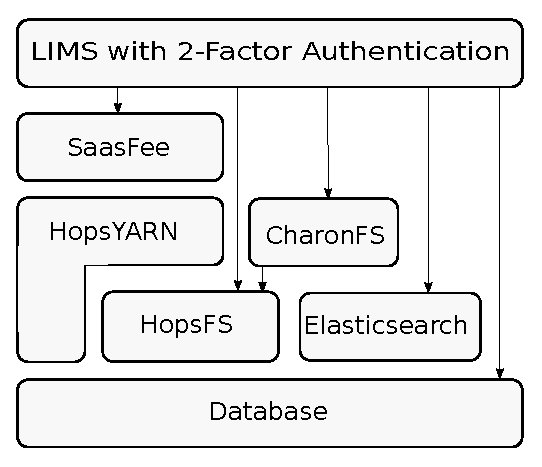
\includegraphics[scale=0.8]{./imgs/stack.eps}
 % stack.eps: 0x0 pixel, 300dpi, 0.00x0.00 cm, bb=0 -1 805 312
 \caption{BiobankCloud Architecture}
 \label{fig:lim}
\end{figure}


BiobankCloud introduces \textbf{DataSets} as a new abstraction to Hadoop, where a DataSet consists of a related group of directories, files, and extended metadata. DataSets can be indexed and searched and are the basic unit of data management in BiobankCloud; all user-generated files or directories belong to a single DataSet. In Biobanking, a sample collection would be a typical example of a DataSet.  To allow for access control of users to DataSets, which is not inherent in the DataSet concept, we introduce the notion of \textbf{Studies}. A Study is a grouping of researchers and DataSets , see figure \ref{fig:studies}. 
% The basic user roles we provide reflect the European Data Protection Directive, with a DataOwner (data controller) and a DataScientist (data processer). DataSets can be shared between Studies (when the necessary security, legal, and ethical conditions for sharing are in place).  In BiobankCloud, we use the access control mechanism of HopsFS to implement the Study- and DataSet-based authorization model. 
% Roles are defined and privileges are enforced in HopsFS.
\begin{figure}[h]
 \centering
 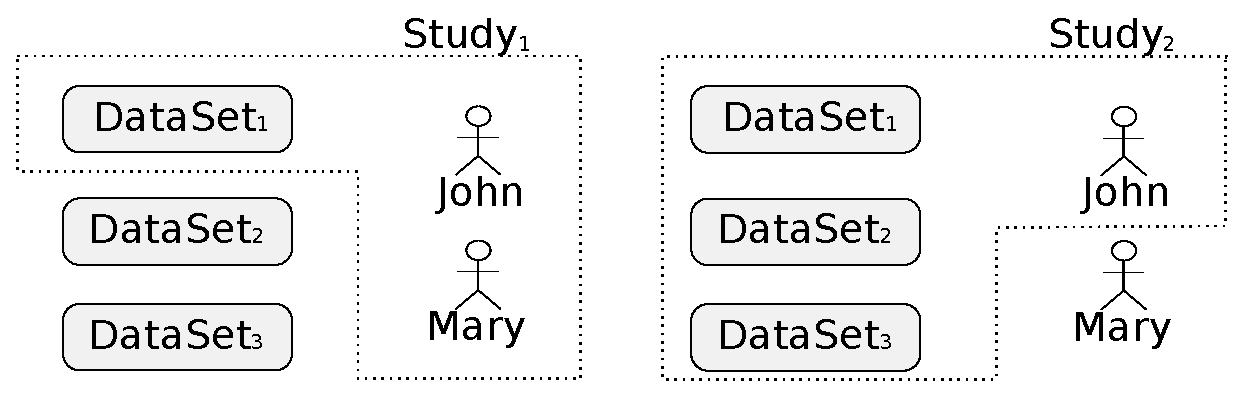
\includegraphics[scale=0.6]{./imgs/projects-as-groupings1.eps}
 % projects-as-groupings1.eps: 0x0 pixel, 300dpi, 0.00x0.00 cm, bb=0 207 582 382
\caption{Study1 has two Users and one DataSet, while Study2 has one User and three DataSets.}
\label{fig:studies}
\end{figure}

%\vskip-5pt
\section{Security Model}

The BiobankCloud environment deploys strong security features for concerns such as confidentiality, integrity and non-repudiation ~\cite{BBCSEC} of data access. This includes authentication, authorization, and auditing. The system allows defining different roles with different access privileges. In designing the system, we applied the Cloud Privacy Threat Modelling~\cite {CPTM} approach to identify the privacy requirements of processing sensitive biomedical data. This model implements a data management policy that aligns with the European data protection directive. The project further implements tools to ensure the correct allocation of legal responsibilities for the data processed within the platform. 


Figure \ref{fig:security} shows the different components of the employed security mechanisms. All BioBankCloud services are protected behind the firewall and only accessible through the secure interfaces over HTTPS channels.

\begin{figure}[h]
\centering
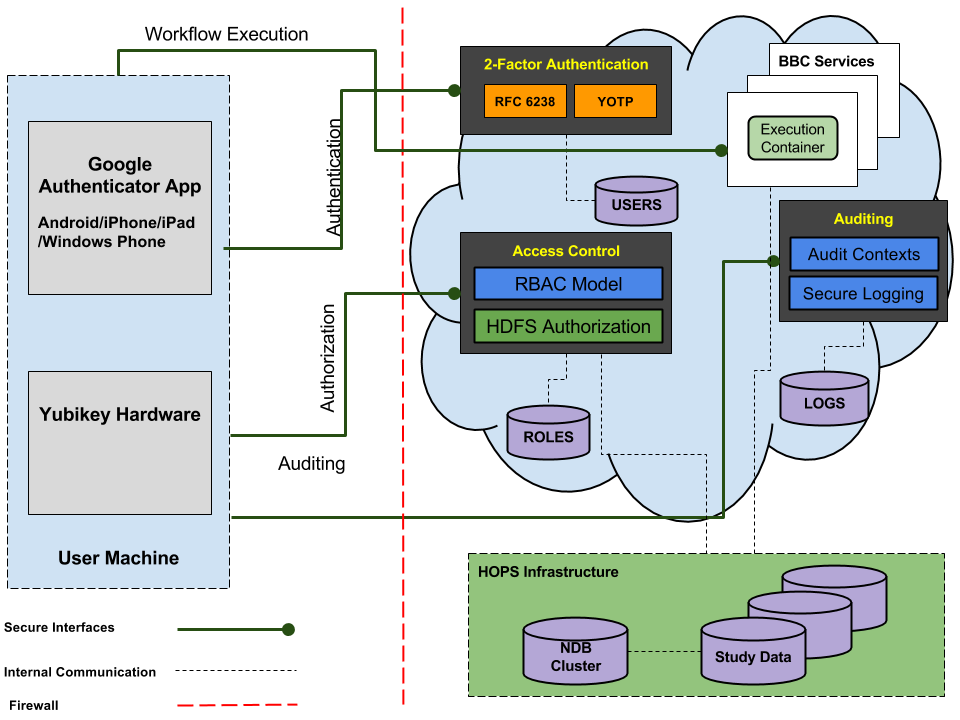
\includegraphics[width=\textwidth]{./imgs/security.png}
\caption{Security framework authorizes access to the BiobankCloud via the web front-end.}
\label{fig:security}
\end{figure}

\subsection{2-Factor Authentication}
The authentication services map the person accessing the platform to a user identity. We provide 2-factor authentication using smart mobile devices or Yubikey \footnote {Yubikey Manual,http://www.yubico.com} hardware tokens to support different groups of users. Users send authentication requests via a Web browser to the authentication service that runs instances of the time-based one-time password (TOTP) and Yubikey one-time password (YOTP) protocols.

In a mobile scenario, a user supplies an one-time generated password by a commercial authenticator in addition to a simple password that was decided during the account registration. The login page authenticates the user to the platform using the TOTP module (Time-Based One-Time Password) as an implementation of the RFC 6238.  In contrast, a Yubikey user would enter the Yubikey device into a USB port. The user enters the simple password that was decided during the account registration and pushes the Yubikey button. The Yubikey login page authenticates the user to the platform via the YOTP module.

\subsection {Role-based Access Control}

The access control component ensures authorized access to all data and services within a platform installation. file system level. Therefore, the system defines several roles\footnote{The concrete roles should be seen as implementations of the European Data Protection Directive.} which are granted certain access rights to certain studies. Examples are a DataOwner (users who may create new data sets), a DataScientist (users who can run workflows on the data), or an auditor (users with access to audit trails for auditing). DataSets technically can be shared between studies, and users may have different roles in different studies. We use the access control mechanism of HopsFS to implement the Study- and DataSet-based authorization model. 


\subsection {Auditing Service}
Finally, the auditing service enables the platform administrator or an external auditor to discover the history of accessing the platform to detect any violation to a policy. It includes several contexts \
such as role, account, study, and login audits. The secure login service assures that actions that are taken by the users are registered for tracing and auditing purposes. Each log event contains informat\
ion such as initiator, target, IP/MAC addresses, timestamp, action, and outcome.

%\vskip-5pt
\section{Hadoop Open Plataform-as-a-Service (Hops)}
In BiobankCloud, we are using our distribution of the Hadoop Filesystem (HDFS), HopsFS, to store genomic data as files.  Hops is a distribution of Apache Hadoop 2 that has a new metadata management architecture based on a shared-nothing, in-memory distributed database, see Figure \ref{fig:hops}. As metadata can now grow to TBs in size (compared to  ~100GB in Apache HDFS \cite{shvachko2010Hdfs}), Hops can scale to store 100s of millions of files.
The HopsFS architecture includes multiple stateless NameNodes that manage the namespace metadata  stored in the database, see figure \ref{subfig:hopsfs}. HopsFS' clients and DataNodes are aware of all NameNodes in the system. HopsFS is  highly available: whenever a NameNode fails the failed operations are automatically retried by clients and the DataNodes by forwarding the failed requests to a different live NameNode. We use MySQL Cluster~\cite{ronstrom2005recovery} as the database, as it has high throughput and is also highly available, although any distributed in-memory database that supports transactions and row level locking could be used. On database node failures, failed transactions are re-scheduled by NameNodes on surviving database nodes.
\begin{figure}[!ht]
    \subfloat[HopsFS\label{subfig:hopsfs}]{%
      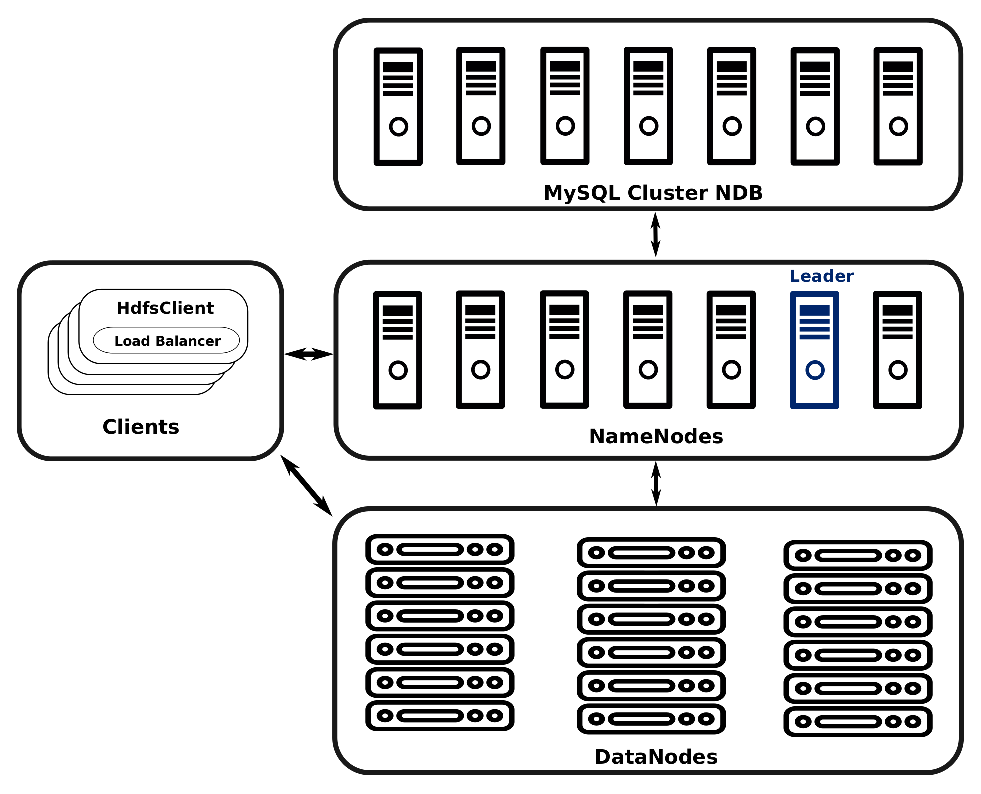
\includegraphics[width=0.46\textwidth]{./imgs/hops-fs-arch.eps}
    }
    \hfill
    \subfloat[HopsYARN\label{subfig:hopsyarn}]{%
      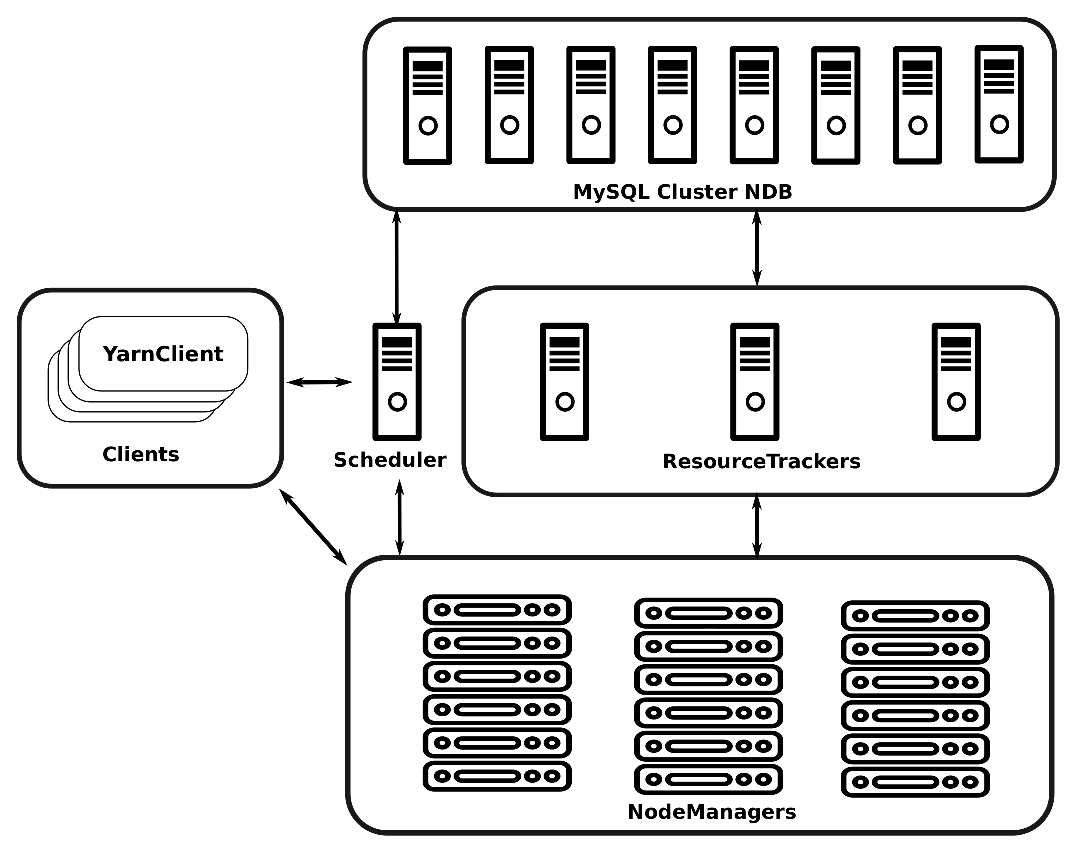
\includegraphics[width=0.47\textwidth]{./imgs/hops-yarn-arch.eps}
    }
    \caption{HopsFS and HopsYARN architectures.}
    \label{fig:hops}
\end{figure}
  
We ensure the consistency of the filesystem metadata by implementing serialized transactions on well-ordered operations on metadata~\cite{hops_consistency}. A leader NameNode is responsible for file system maintenance tasks,  and leader failure triggers our own leader-election service based on the database~\cite{hopselection}. 
HopsFS can reduce the amount of storage space required to store genomic data, while maintaining high availability by storing files using Reed-Solomon erasure coding, instead of the traditional three-way replication  used in HDFS. Erasure-coding can reduce disk space consumption by 44\% compared to three-way replication. In HopsFS, an ErasureCodingManager runs on the  leader NameNode, managing file encoding and file repair operations, as well as implementing a policy that places file blocks on DataNodes in such a way that ensures that, in the event of a DataNode failure, affected files can still be repaired.

\subsection*{Designing, Indexing and Searching Extended Metadata}
We store genomes in HopsFS. However, Biobanks require much more extensive metadata for genomes than is available for HDFS files. The limited metadata available in HDFS files includes file size, time last modified and owner. We also need information such as the sample and sample collection the genome belongs to, the type of sample, and donor information. Our LIMS provides a UI tool for Biobankers who are not programmers to design their own  extended metadata that is linked  to genomes, sample collections, DataSets or Studies. This extended metadata is stored in the same database as the file system metadata and the integrity of the extended metadata is guaranteed using foreign keys to the file or directory the metadata refers to.
To make this extended metadata searchable, we asynchronously and transparently replicate it to Elasticsearch. This indexing of extended metadata enables free-text searching for samples.


\subsection*{HopsYARN}
HopsYARN is our implementation of Apache YARN, in which we have (again) migrated the metadata to MySQL Cluster. We partitioned YARN's ResourceManager into (1) ResourceTracker nodes that process heartbeats from and send commands to NodeManagers, and (2) a single scheduler node that implements all other ResourceManager services, see Figure \ref{fig:hops}. If the scheduler node fails, our leader election service will elect a ResourceTracker node as the new scheduler that then loads the scheduler state from the database. HopsYARN scales to handle larger clusters than Apache YARN as resource tracking has been offloaded from the scheduler node to other nodes, and resource tracking traffic grows linearly with cluster size. This will, in time, enable larger numbers of genomes to be analyzed in a single system.


%\vskip-5pt
\section{SAASFEE}
\label{saasfee}

%one page, should include an evaluation (see Introduction)
%one paragraph on saasfee (possibly w/ img)
%one paragraph on hiway
%one paragraph on cuneiform
%one paragraph on evaluation (w/ image)
% \vspace{-5mm}

To process the vast amounts of genomic data stored in today's biobanks, researchers have a diverse ecosystem of tools at their disposal~\cite{Pabinger2014}. Depending on the research question at hand, these tools are often used in conjunction with one another, resulting in complex and intertwined analysis pipelines. Scientific workflow management systems (SWfMSs) facilitate the design, refinement, execution, monitoring, sharing, and maintenance of such analysis pipelines. SAASFEE~\cite{vldb_demo} is a SWfMS that supports the scalable execution of arbitrarily complex workflows. It encompasses the functional workflow language Cuneiform as well as Hi-WAY, a higher-level scheduler for both Hadoop YARN and HopsYARN. See Figure~\ref{fig:saasfee_stack} for the complete software stack of SAASFEE.

\begin{figure}
  \centering
  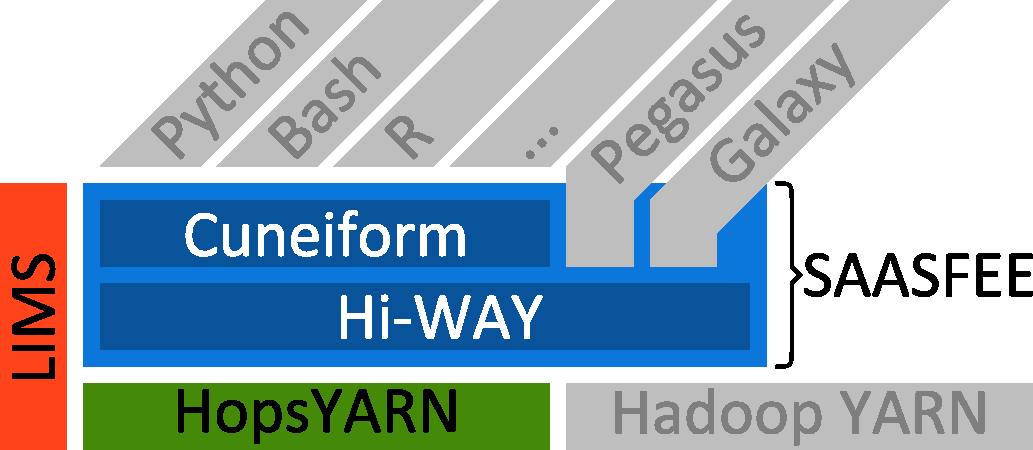
\includegraphics[width=.67\textwidth]{imgs/saasfee_stack.pdf}
  \caption{The software stack of the scientific workflow management system SAASFEE, which comprises the functional workflow language Cuneiform as well as the Hi-WAY workflow scheduler for Hadoop. Cuneiform can execute foreign code written in languages like Python, Bash, and R. Besides Cuneiform, Hi-WAY can also interpret the workflow languages of the SWfMSs Pegasus and Galaxy. SAASFEE can be run both on Hops as well as Apache Hadoop. SAASFEE and HopsYARN can be interfaced and configured via the web interface provided by the LIMS.}
  \label{fig:saasfee_stack}
\end{figure}

Analysis pipelines for large-scale genomic data employ many different software tools and libraries with diverse Application Programming Interfaces (APIs). At the same time the growing amounts of data to be analyzed necessitate parallel and distributed execution of these analysis pipelines. Thus, the methods for specifying such analysis pipelines need to meet both concerns -- integration and parallelism equally. The functional workflow Language Cuneiform has been designed to meet these requirements~\cite{Brandt2015}. Cuneiform allows the integration of software tools and libraries with APIs in many different programming languages. This way, command-line tools (e.g., Bowtie~\cite{langmead2009ultrafast}) can be integrated with similar ease as, for instance, R libraries (e.g., CummeRbund~\cite{goff2012cummerbund}). By partitioning large data sets and processing these partitions in parallel, data parallelism can be exploited in addition to task parallelism to speed up computation. Cuneiform automatically detects and exploits data and task parallelism in a workflow specification. Editing and debugging workflows is supported by the tools and visualization features provided with the Cuneiform interpreter.

Hi-WAY is a higher-level scheduler that enables the execution of scientific workflows on top of YARN. Hi-WAY executes each of the tasks comprising the workflow in a separate container, which is the basic unit of computation in YARN. Input, output and intermediate files created during workflow execution are stored in Hadoop's distributed file system HDFS. Consequently, Hi-WAY benefits form the fault-tolerance and scalability of the Hadoop ecosystem. It has been evaluated to scale to more than 600 concurrent tasks.

Hi-WAY provides a selection of established scheduling policies conducting task placement based on
\begin{inparaenum}[(a)]
  \item the locality of a task's input data to diminish network load and
  \item task runtime estimation based on past measurements to utilize resources efficiently.
\end{inparaenum}
To enable repeatability of experiments, Hi-WAY generates exhaustive provenance traces during workflow execution, which can be shared and re-executed or archived in a database. One of the major distinctive features of SAASFEE is its strong emphasis on integration of external software. This is true for both Cuneiform, which is able to integrate foreign code and command-line tools, and Hi-WAY, which is capable of running not only Cuneiform workflows, but also workflows designed in the SWfMSs Pegasus~\cite{pegasus_fgcs} and Galaxy~\cite{Goecks10}.


%% Example workflow %%%%%%%%

\begin{figure}
  \centering
  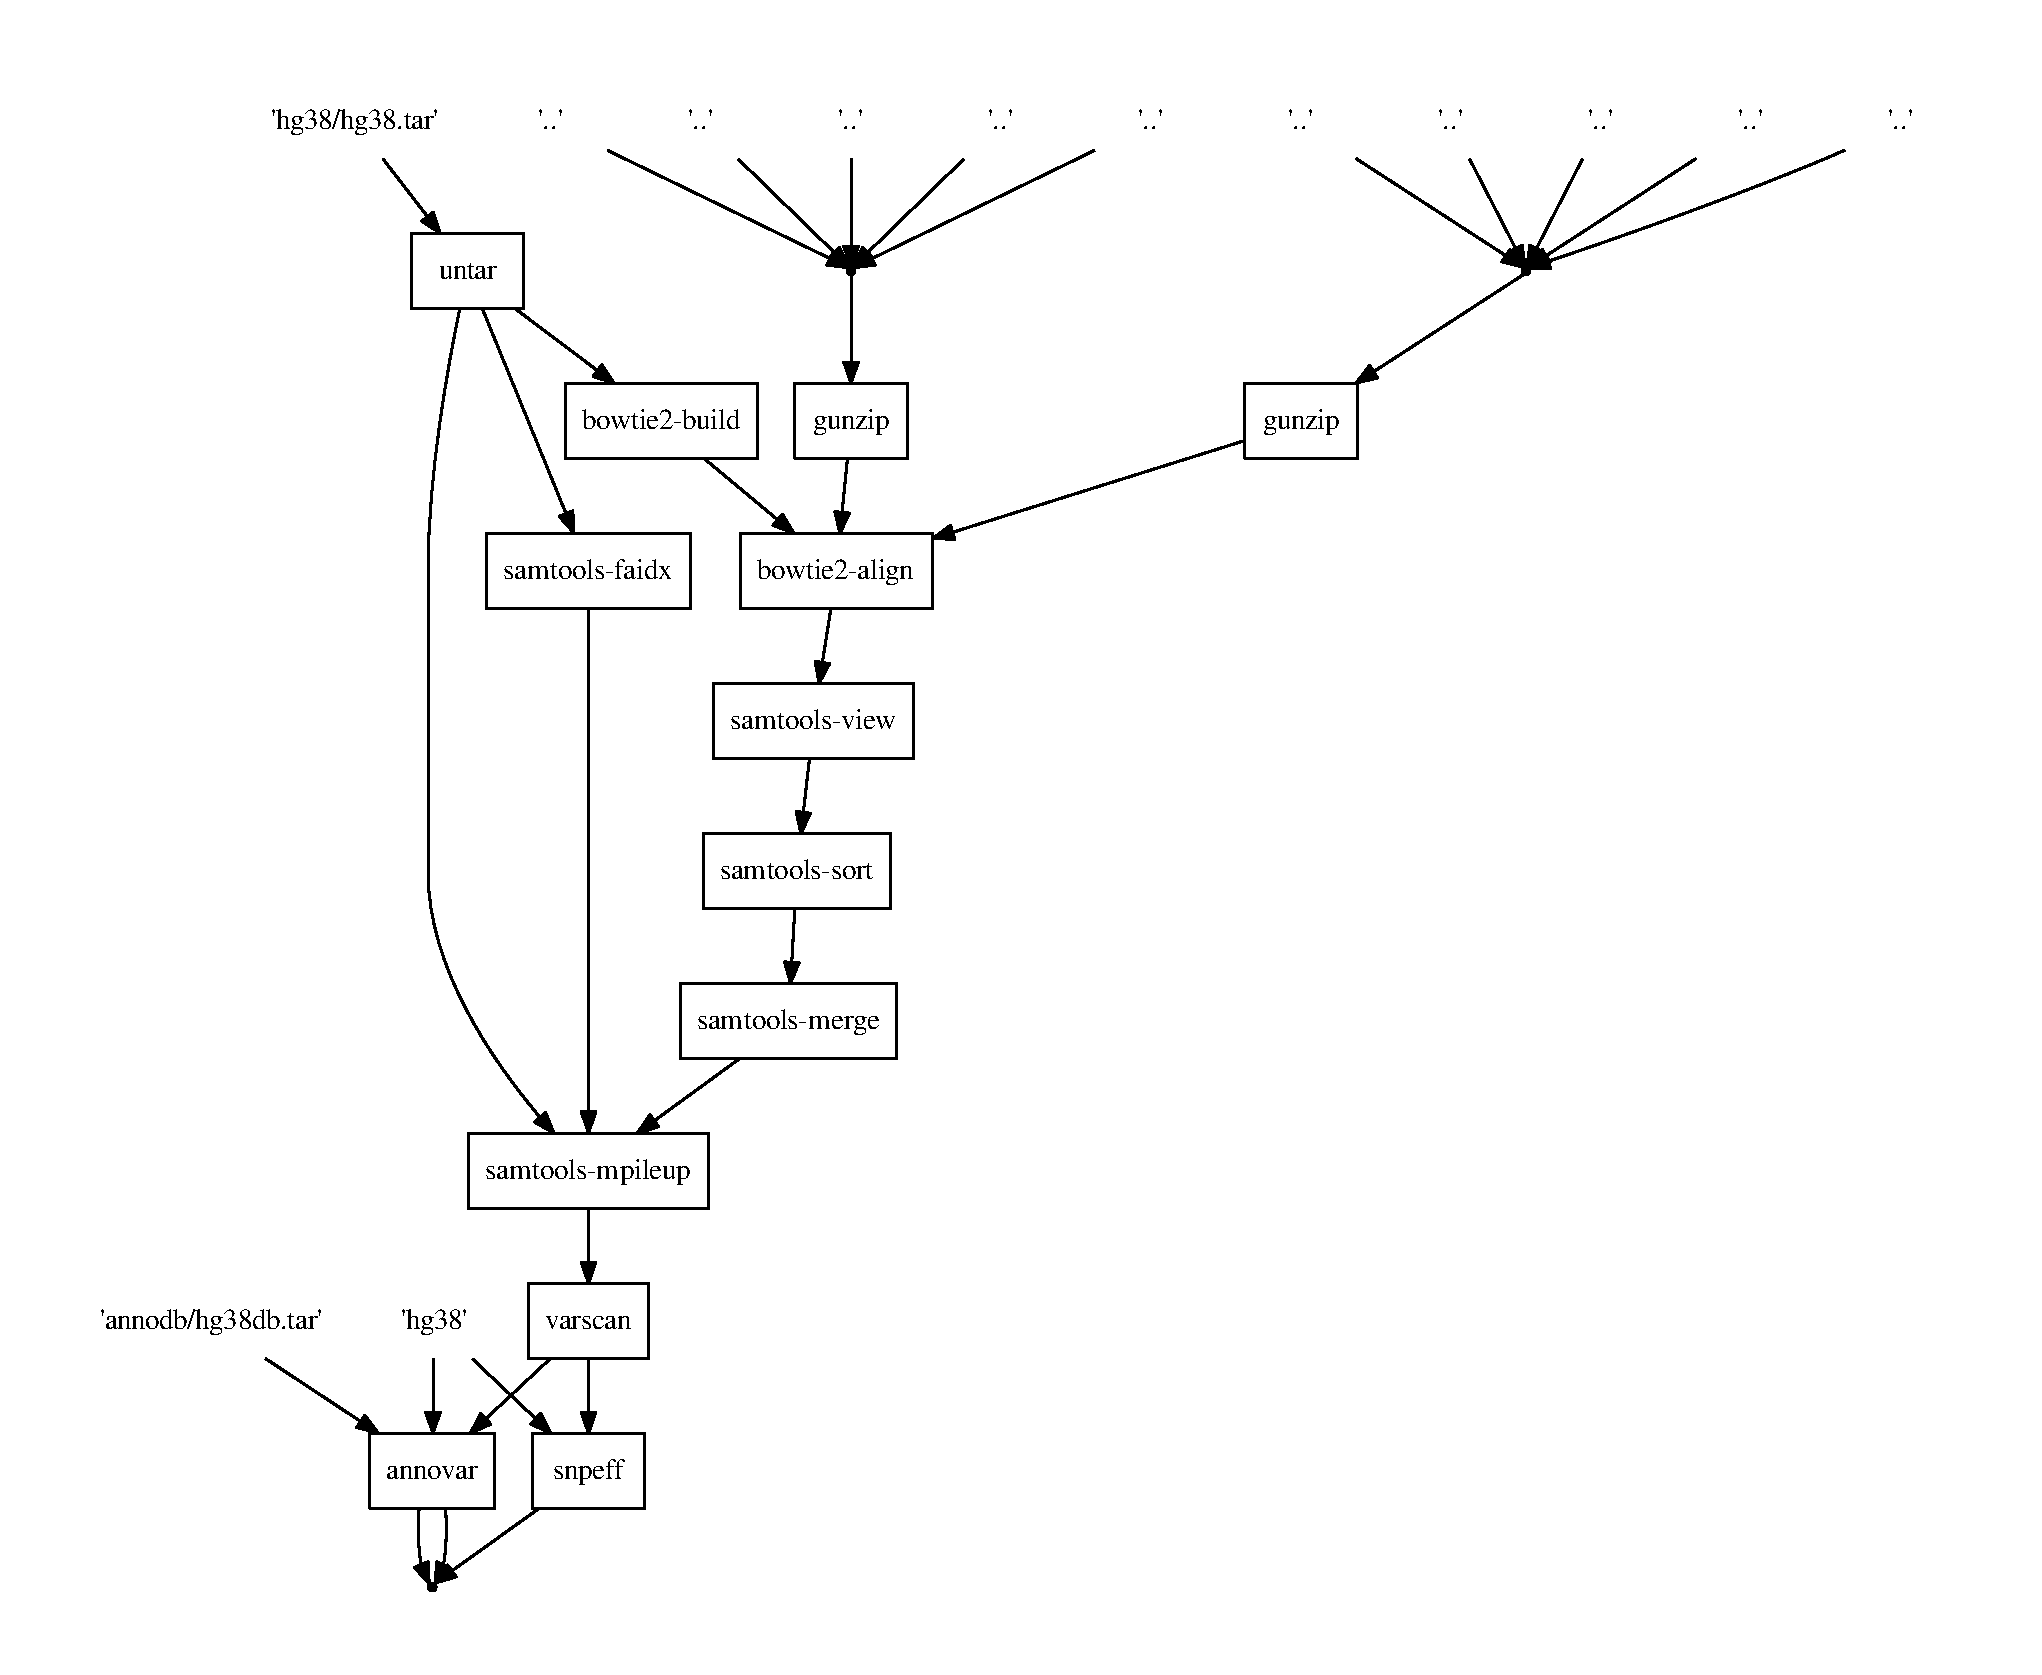
\includegraphics[width=.85\textwidth]{imgs/variant_call11b.pdf}
  \caption{Static call graph of variant calling workflow. Box-shaped nodes represent distinct tasks, edges represent data dependencies.}
  \label{fig:variant_call}
\end{figure}

We demonstrate the applicability of SAASFEE for large-scale biobank use cases by discussing an example workflow for variant calling. In this use case we try to discover differences in the genome of an organism in comparison to a reference genome. Furthermore, the discovered differences are annotated with database information to ease their interpretation by a specialist. Figure \ref{fig:variant_call} shows the static call graph for this workflow which was automatically derived from the workflow script written in Cuneiform. It enumerates the different data processing steps and gives a coarse overview of task dependencies. Each of these tasks integrates a different command-line tool which is wrapped in Cuneiform and called like a function. The workflow is extensible in the way that each intermediate result can serve as the input to a new sub-workflow and tools can be differently parametrized and, if file formats are standardized, exchanged with different tools.



%%%%%%%%%%%%%%%%%%%%%%%%%%%%

As a first step to test the scalability of SAASFEE for large-scale use cases which are relevant for biobanks, we ran this variant calling pipeline on 10~GB of compressed whole genome sequencing reads from the 1000 Genomes Project. These reads were aligned against a reference genome, variants were called, and the resulting sets of variants were annotated using publicly available databases. Figure~\ref{fig:saasfee_scaling} shows the scalability of this workflow. Within the limits of the setup chosen, linear scaling behavior could be achieved for the variant calling workflow.

\begin{figure}
  \centering
  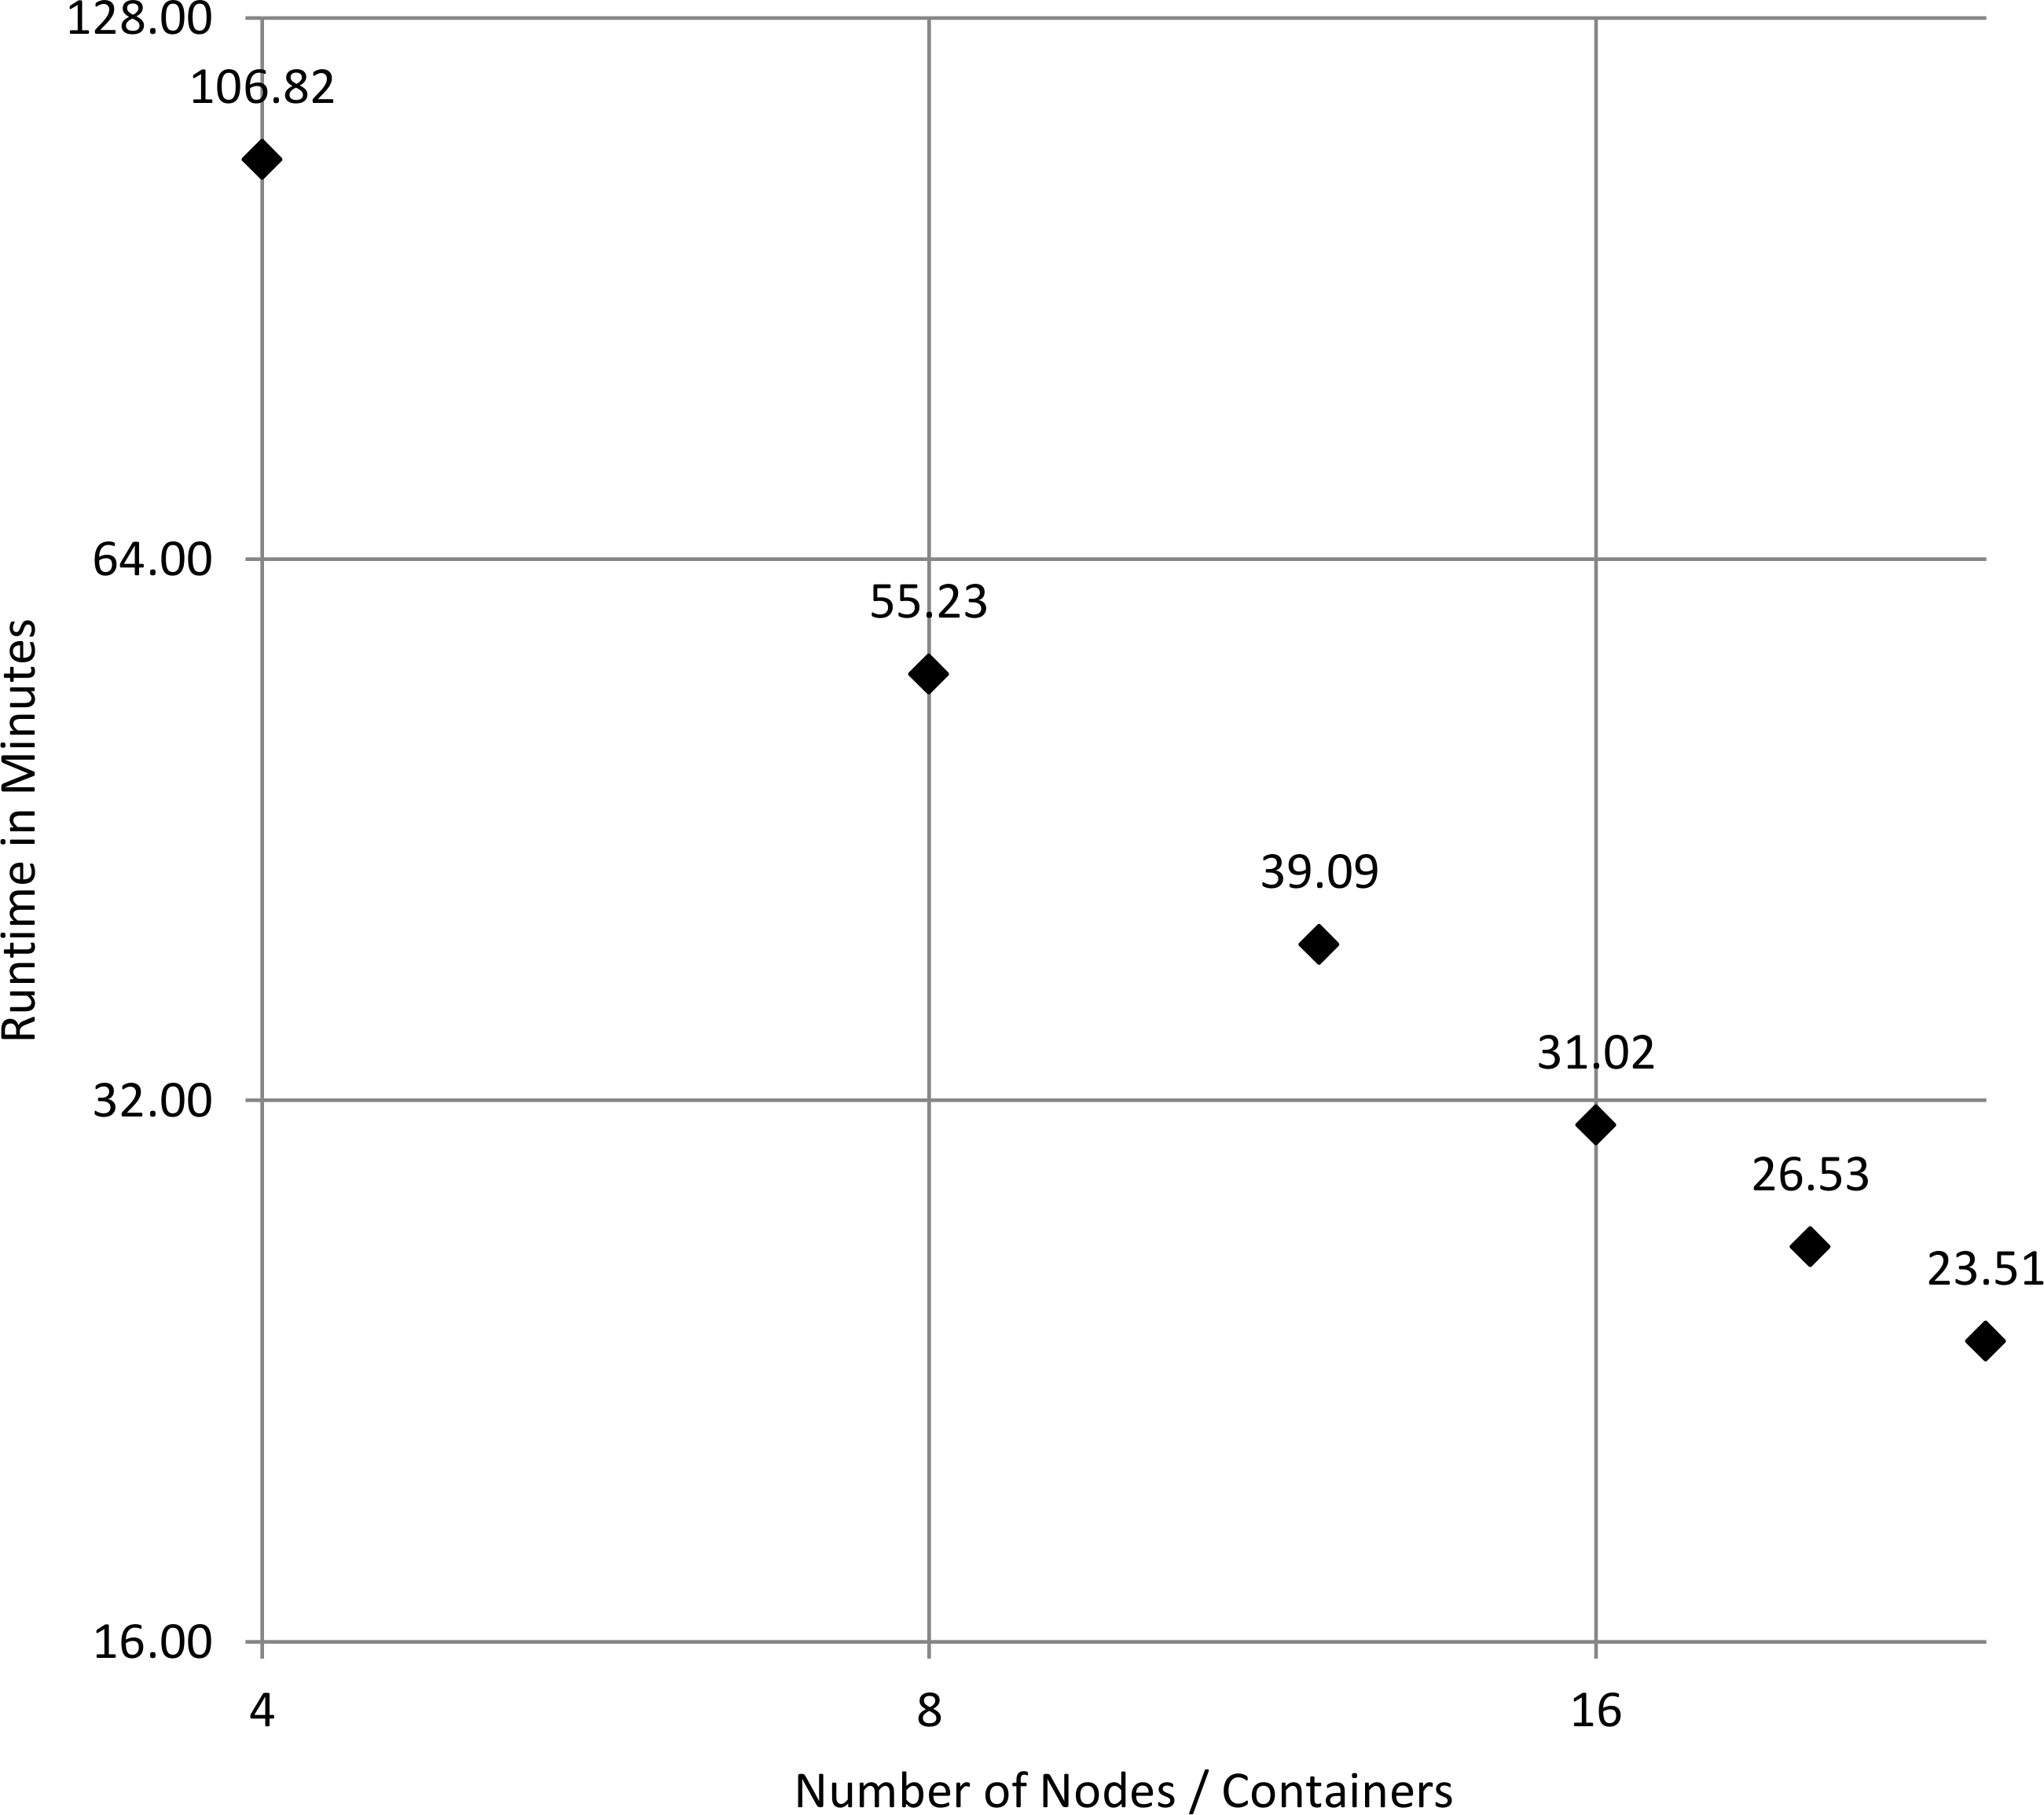
\includegraphics[width=.55\textwidth]{imgs/wf_runtime.png}
  \caption{Scalability experiment for the SAASFEE software stack. A variant calling workflow has been scaled out on up to 24 nodes. Both axes, the runtime in minutes and the number of nodes are on a logarithmic scale (published in Brandt et al. 2015~\cite{Brandt2015}).}
  \label{fig:saasfee_scaling}
\end{figure}
\vspace{-5mm}

%\vskip-5pt
\section{Workflows implemented in BiobankCloud}
Next generation sequencing, a technology first introduced to the market in 2005, has revolutionized biological research during the last ten years~\cite{shendure2008next}. The technology allows scientist to study not only the genome of any species, but also the transcriptome and the epigenome.
We have implemented several pipelines for the analysis of the most common types of next generation sequencing data into the BiobankCloud. 

\textbf{Variant Calling pipeline:} Genetic variations represent changes in the order of the bases in a DNA sequence and variations in the human genome play a decisive role in human disease. The most common variations in the genome are the single nucleotide variations and short insertions and deletions. For this pipeline whole genome sequencing and/or whole exome sequencing data can be chosen as input data and the workflow was derived from Thalheim \cite{snp_wf_thalheim}. Figure \ref{fig:workflow_snp} shows a schematic overview on this Variant Calling pipeline built in BiobankCloud.


\vskip-5pt
\begin{figure}[h]
\centering
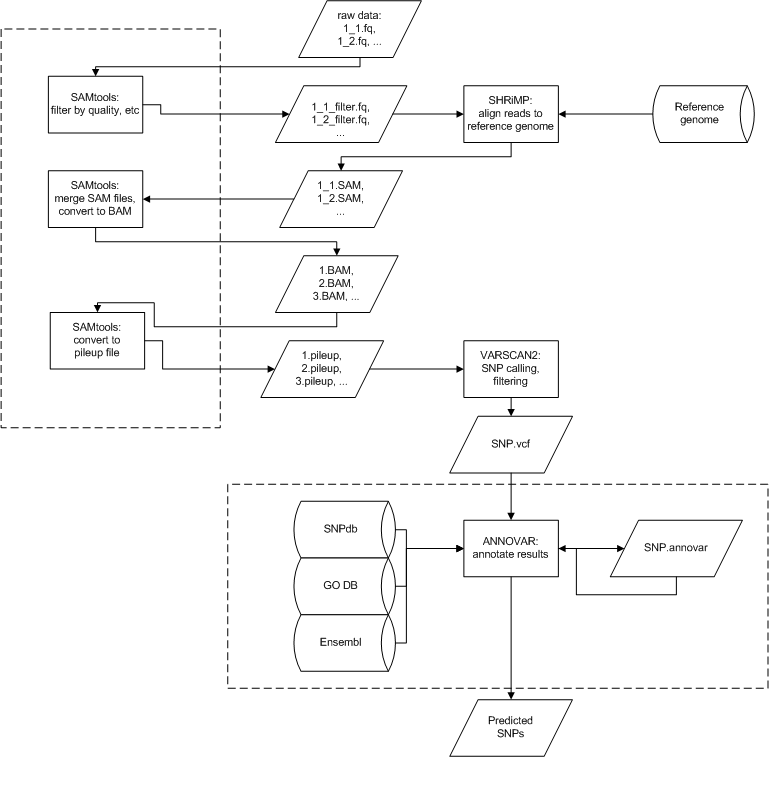
\includegraphics[width=0.6\textwidth]{./imgs/wf_snp.png}
\caption{Subsequent processing steps in BiobankCloud's Variant Calling pipeline.}
\label{fig:workflow_snp}
\end{figure}
\vskip-5pt


\textbf{Gene Expression pipeline:} This pipeline uses RNA-Seq data as input and enables the user to study differential expression on different levels such as 
genes and transcripts. Furthermore, it detects differential splicing and promoter use between two or more groups of interest.
The pipeline was implemented according to Trapnell et al.\cite{trapnell2012differential, trapnell2013differential}.

\textbf{ChIP-Seq pipeline:} ChIP-Seq (Chromatin immunoprecipitation coupled with high-throughput sequencing) is the standard technique for studying the genome-wide binding profiles of DNA-binding proteins, e.g. transcription factors, as well as the distribution of histone modifications. ChIP-Seq NGS data are the input data for this pipeline and the workflow described by Dimitrova et al. \cite{dimitrova2014pax5} was used.

\textbf{microRNA pipeline:} microRNAs are short expressed RNAs that play a key role in many biological processes and in different diseases. Our pipeline for analysis of the expression profiles of microRNAs is based on the publication of Kozubek et al. \cite{kozubek2013depth} and is using small RNA-Seq data as input.





%\vskip-5pt
\section{Sharing Data Between Clusters with CharonFS}
\label{charonfs}
\textsc{Charon} is a cloud-backed file system capable of storing and sharing big data in a secure, reliable, and efficient way using multiple cloud providers and storage repositories. 
It is secure and reliable because it does not require trust on any single entity, and it supports the storage of different types of data in distinct locations to comply with required privacy premises. 
Two distinguishing features of \textsc{Charon} are its serverless design (no client-managed server is required in the cloud) and its efficient management of large files (by employing prefetching, cache, and background writes).

Figure~\ref{fig:charon} illustrates a deployment scenario where two biobanks store their data in local repositories, in single public cloud providers, and in a resilient cloud-of-clouds. 
In this scenario, the namespace tree has six nodes: directories \texttt{d1} and \texttt{d2}, and files \texttt{A}, \texttt{B}, \texttt{C}, and \texttt{D}. 
The namespace is maintained in the cloud-of-clouds, together with file \texttt{B}.
File \texttt{D}, less critical, is kept in a single cloud.
File \texttt{A} is stored locally because it cannot leave Biobank 2. 
File \texttt{C} is shared between the two sites (e.g., in the same country), thus being stored in both of them.

% \vspace{-5mm}
\begin{figure}[ht]
 \centering
 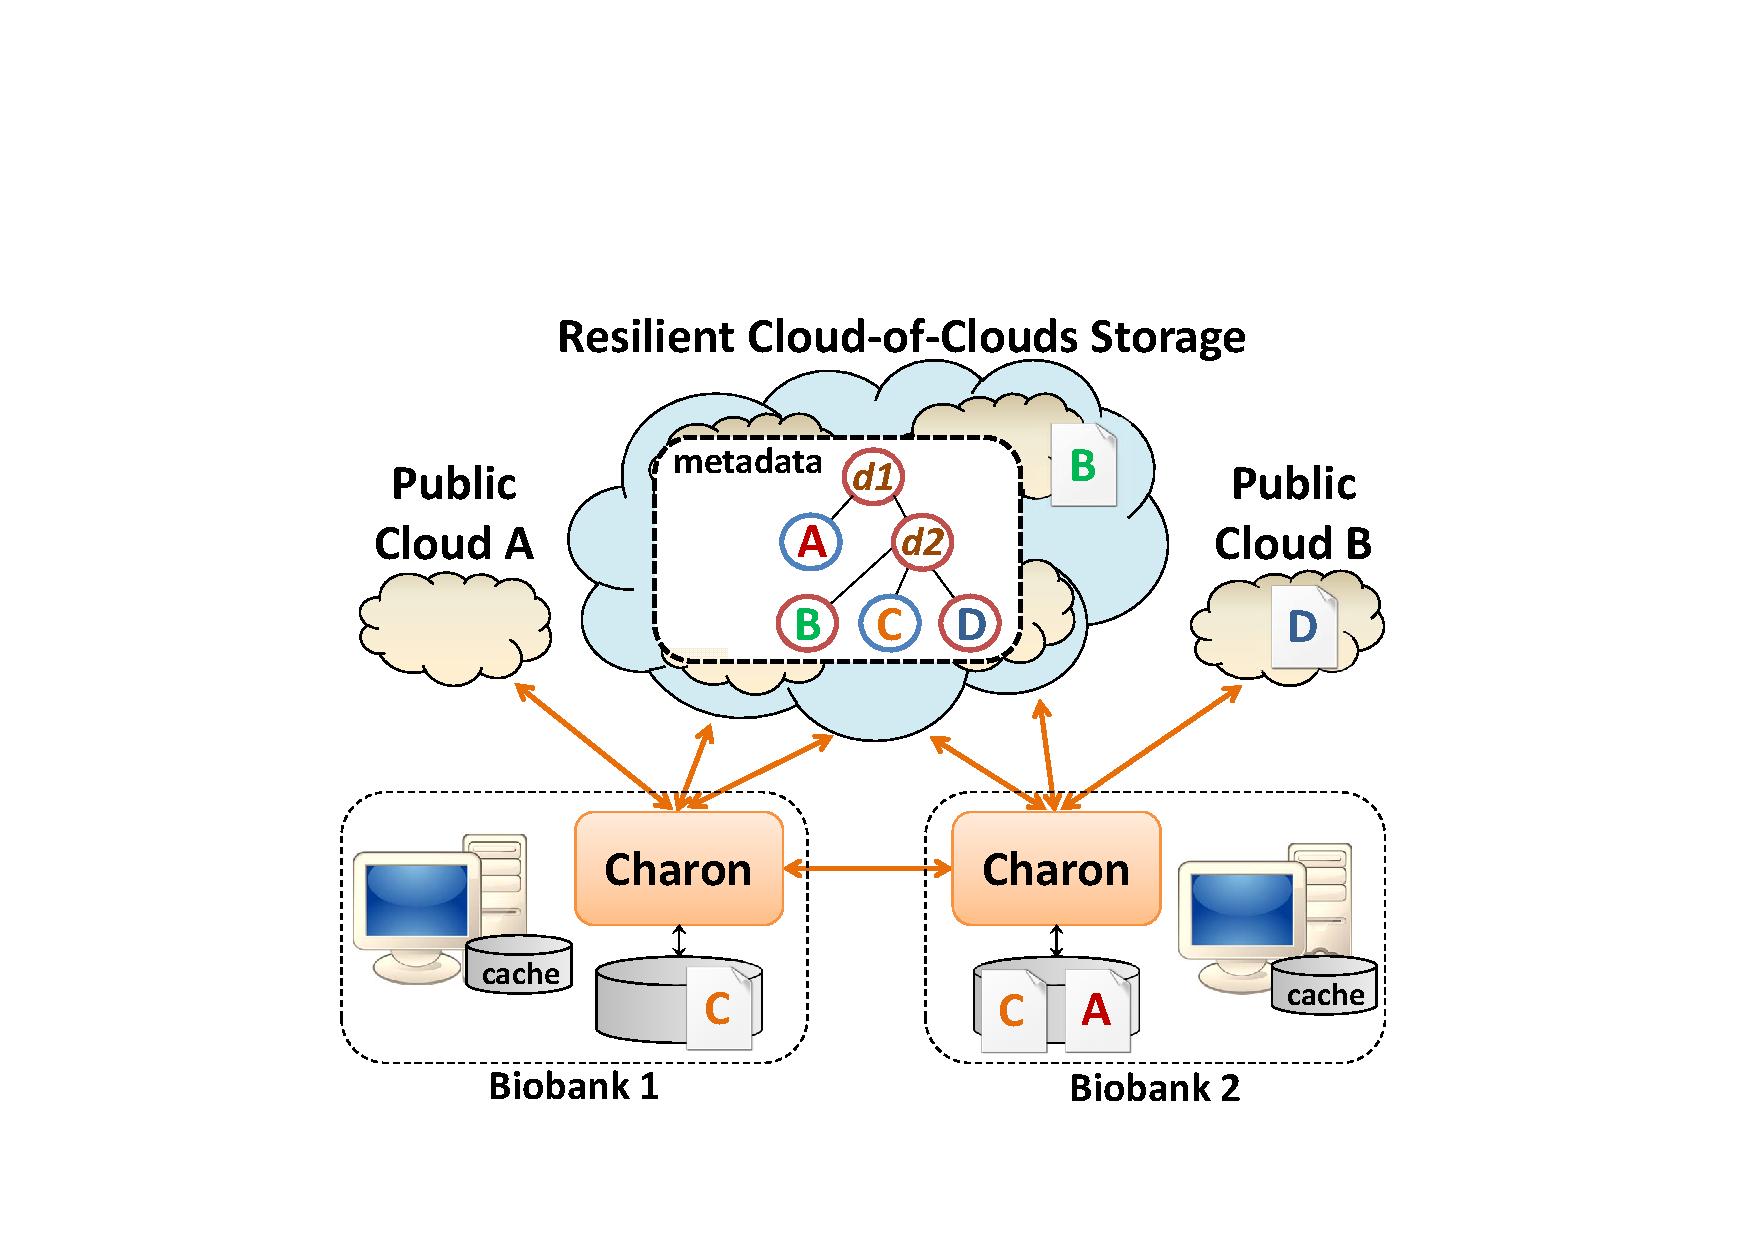
\includegraphics[width=0.5\columnwidth]{./imgs/charon_arch.pdf}
 % charon_arch.pdf: 0x0 pixel, 300dpi, 0.00x0.00 cm, bb=
\caption{\small \textsc{Charon} overview.}
\label{fig:charon}
\end{figure}
% \vspace{-5mm}

The BiobankCloud platform is able to process data stored in HopsFS, which has a view of all data being stored in a single cluster. \textsc{Charon} performs the inter-datacenter tasks and the processes between Biobanks and public clouds.
% In the next section, we discuss the integration between these two storage systems and evaluate the most appropriate integration scenario for the BiobankCloud platform.

% \vskip-5pt
\section{Automated Installation}

BiobankCloud supports automated installation. It can be installed by non-technical users who can click-through an installation using only a file that defines a BiobankCloud cluster and account credentials for a cloud computing platform. Our solution is based both the configuration management platform Chef~\cite{chef13nelson}, and an orchestration engine that we designed for Chef called Karamel. The main reason we adopted Chef is that it provides support for both upgrading long-lived stateful software and parameterized installations. This contrasts with container-based approaches, such as Docker, that are not yet suitable for online upgrading of stateful systems and also have limited support for parameterization and orchestration. Chef has, however, no support for orchestrating installations. For distributed systems with many services, such as BiobankCloud, there is often a need to start and initialize services in a well-defined order, that is, to orchestrate the installation and starting of services. To this end, we developed an orchestration engine for Chef called Karamel. 

In Chef, the basic unit of installation is a recipe, a program written in a domain-specifc language for Ruby. In keeping with best practice, in BiobankCloud, each recipe corresponds to a single distributed system service. Recipes are grouped together into software artifacts called cookbooks. We have written Chef cookbooks and services for all our software components. our Hadoop platform stores its single cookbook in a repository on GitHub called \textit{hops-hadoop-chef}. For each Hadoop services, our hops cookbook has recipe that both installs starts it. The recipes include the NameNode (hops::nn), the DataNode (hops::dn), ResourceManager (hops::rm), and NodeManager (hops::nm). Hops also uses a database called NDB, with its cookbook stored in ndb-chef. Similarly, our LIMS (hopsworks) and SAASFEE (hiway) have their own repositories. Karamel aaugments cookbooks with orchestration rules for recipes defined in a file called \textit{Karamelfile}. The Karamelfile defines what services need to be running within the cluster (and locally) before a given recipe is executed. 

Given the set of all recipes that need to be installed on all nodes, as weel as the orchestration rules for the cookbooks, Karamel can take a declarative cluster definition and execute it to install the BiobankCloud platform. In listing~\ref{yaml} below, we can see a definition of a large BiobankCloud cluster, consisting of 110 nodes. The cluster is defined for Amazon Web Services (\textit{ec2}), but that section of the file can be modified to deploy the same cluster to a different cloud platform, such as OpenStack. The \textit{cookbooks} section defines where the cookbook software artifacts are located. Karamel uses this information to download orchestration rules for the cookbooks and metadata, thus enabling smaller cluster definition files, since they do not need their own orchestration rules. The \textit{attrs} section defines a single parameter for the user that will run the LIMS. In production installations, the \textit{attrs} section typically contains more extensive configuration parameters. Finally the \textit{groups} section defines groups of nodes that install the same software stack. The software stack for each group is defined as a list of recipes. Here, we have four different groups: one for the frontend LIMS (ui), one for the Hadoop and database management services (mgmtnodes), one for the database (datanodes), and one for the storage and processing nodes (workers).

% \begin{lstlisting}[language=yaml,frame=shadowbox,label=karamel-cluster,caption=Karamel Cluster Definition for BiobankCloud,float=t]
\begin{lstlisting}[frame=shadowbox,label=karamel-cluster,caption=Karamel Cluster Definition for BiobankCloud,float=t]
name: BiobankCloud
ec2:
    type: m3.medium
    region: eu-west-1

cookbooks:
  ndb: 
    github: "hopshadoop/ndb-chef"
  hops: 
    github: "hopshadoop/hops-hadoop-chef"
  hopsworks: 
    github: "hopshadoop/hopsworks-chef"
  hiway: 
    github: "biobankcloud/hiway-chef"
    
attrs:
  hopsworks:
    user: bbc
    
groups: 
  ui:
    size: 4
    recipes: 
        - hopsworks, hiway::client
  mgmtnodes:
    size: 4
    recipes: 
        - hops::nn, hops::rm, ndb::mgmd, ndb::mysqld
  datanodes:
    size: 2
    recipes: 
        - ndb::ndbd
  workers:
    size: 100
    recipes: 
        - hops::dn, hops::nm, hiway::worker
\end{lstlisting}\label{yaml}


\section{Conclusions}
In this paper, we introduced the BiobankCloud platform, a platform that provides a number of features necessary for biobanks to adopt Hadoop-based solutions for managing NGS data. Critical security features that we have introduced for managing sensitive data include multi-tenancy to isolate Studies and 2-factor authentication. Next-generation data management systems for NGS data must be massively scalable. We introduced our scalable storage service, HopsFS, our processing framework, HopsYARN, and our framework for scalable bioinformatics workflows, SAASFEE. We also provide metadata design and search services, while ensuring the integrity of metadata. Finally, in Charon, we showed how we can leverage public clouds to share data securely between clusters. BiobankCloud's secure and scalable open platform software is helping to remove the biobank bottleneck and enable population-level genomics.
% \vskip-5pt
\section{Acknowledgements}
This work is funded by the EU FP7 project ``Scalable, Secure Storage and Analysis of Biobank Data'' under Grant Agreement no. 317871. 
%\vskip-5pt
\bibliographystyle{ieeetr}
\bibliography{bbc-dmah15}

\end{document}
